% Options for packages loaded elsewhere
\PassOptionsToPackage{unicode}{hyperref}
\PassOptionsToPackage{hyphens}{url}
%
\documentclass[
]{article}
\usepackage{lmodern}
\usepackage{amssymb,amsmath}
\usepackage{ifxetex,ifluatex}
\ifnum 0\ifxetex 1\fi\ifluatex 1\fi=0 % if pdftex
  \usepackage[T1]{fontenc}
  \usepackage[utf8]{inputenc}
  \usepackage{textcomp} % provide euro and other symbols
\else % if luatex or xetex
  \usepackage{unicode-math}
  \defaultfontfeatures{Scale=MatchLowercase}
  \defaultfontfeatures[\rmfamily]{Ligatures=TeX,Scale=1}
\fi
% Use upquote if available, for straight quotes in verbatim environments
\IfFileExists{upquote.sty}{\usepackage{upquote}}{}
\IfFileExists{microtype.sty}{% use microtype if available
  \usepackage[]{microtype}
  \UseMicrotypeSet[protrusion]{basicmath} % disable protrusion for tt fonts
}{}
\makeatletter
\@ifundefined{KOMAClassName}{% if non-KOMA class
  \IfFileExists{parskip.sty}{%
    \usepackage{parskip}
  }{% else
    \setlength{\parindent}{0pt}
    \setlength{\parskip}{6pt plus 2pt minus 1pt}}
}{% if KOMA class
  \KOMAoptions{parskip=half}}
\makeatother
\usepackage{xcolor}
\IfFileExists{xurl.sty}{\usepackage{xurl}}{} % add URL line breaks if available
\IfFileExists{bookmark.sty}{\usepackage{bookmark}}{\usepackage{hyperref}}
\hypersetup{
  hidelinks,
  pdfcreator={LaTeX via pandoc}}
\urlstyle{same} % disable monospaced font for URLs
\usepackage{graphicx}
\makeatletter
\def\maxwidth{\ifdim\Gin@nat@width>\linewidth\linewidth\else\Gin@nat@width\fi}
\def\maxheight{\ifdim\Gin@nat@height>\textheight\textheight\else\Gin@nat@height\fi}
\makeatother
% Scale images if necessary, so that they will not overflow the page
% margins by default, and it is still possible to overwrite the defaults
% using explicit options in \includegraphics[width, height, ...]{}
\setkeys{Gin}{width=\maxwidth,height=\maxheight,keepaspectratio}
% Set default figure placement to htbp
\makeatletter
\def\fps@figure{htbp}
\makeatother
\setlength{\emergencystretch}{3em} % prevent overfull lines
\providecommand{\tightlist}{%
  \setlength{\itemsep}{0pt}\setlength{\parskip}{0pt}}
\setcounter{secnumdepth}{-\maxdimen} % remove section numbering

\author{}
\date{}

\begin{document}

\hypertarget{stage-m2r}{%
\section{Stage M2R}\label{stage-m2r}}

Greg McShane 2019-2020

\href{https://macbuse.github.io/}{my webpage}

\hypertarget{context}{%
\subsection{Context}\label{context}}

The moduli space of Riemann surfaces is a very old and rich subject. The
connexion with hyperbolic geometry was recognised by Klein as being of
great importance and through the work of Thurston, Penner and many
others at the end of the last century has improved our understanding of
the geometry of Teichmueller space, the mapping class group and the
moduli space itself. One important development has been the discovery of
Mirzakhani's volume polynomials, the recursion they satisfy and the
resulting formulation of so-called
\href{https://arxiv.org/abs/1711.04729}{geometric recursion}.

\begin{figure}
\centering
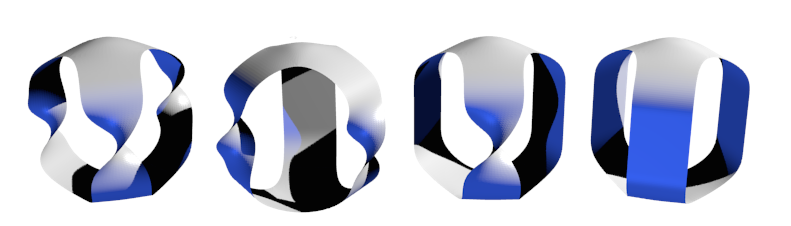
\includegraphics{./4surfaces.png}
\caption{Orientable and non orientable surfaces}
\end{figure}

The Figure show the one holed torus, one holed Klein bottle, two holed
projective plane and the three holed sphere.

A \href{https://en.wikipedia.org/wiki/Klein_surface}{Klein surface} is a
non orientable topological surface together with a hyperbolic structure.
The moduli space of Klein surfaces is much less well understood than
that of Riemann surfaces. In particular there seems to be no notion of
Mirzakhani's polynomials for Klein surfaces nor asymptotic formula for
the number of closed simple geodesics.

In a \href{https://arxiv.org/abs/1706.08798}{recent manuscript}
Gendulphe hakes some calculations and proposes an explanation as to why
there can be no such polynomials they should not exist. In another
\href{https://arxiv.org/abs/1705.09377}{work} Magee proves a counting
formula for counting one sided simple closed geodesics on Fuchsian
thrice punctured projective planes showing surprisingly that the growth
rate is not polynomial.

\hypertarget{details-of-the-stage}{%
\subsection{Details of the stage}\label{details-of-the-stage}}

We will review the basic geometric constructions used in the oriented
case and see how they have to be modified in the article of PAPADOPOULOS
and PENNER. Next we will study the character variety for small surfaces
as in Goldman, et al. Finally we will go through Gendulphe and compare
hs results with that of Magee to see why there are no polynomials.

\hypertarget{references}{%
\subsection{References}\label{references}}

\begin{enumerate}
\def\labelenumi{\arabic{enumi}.}
\tightlist
\item
  Lengths of geodesics on non-orientable hyperbolic surfaces
  \textbf{Paul Norbury}
  \href{https://arxiv.org/abs/math/0612128}{Preprint}
\item
  What's wrong with the growth of simple closed geodesics on
  nonorientable hyperbolic surfaces \textbf{Matthieu Gendulphe}
  \href{https://arxiv.org/abs/1705.09377}{Preprint
  arxiv.org/abs/1705.09377}
\item
  Automorphisms of two-generator free groups and spaces of isometric
  actions on the hyperbolic plane \textbf{William Goldman, et al.}
  \href{https://arxiv.org/abs/1509.03790}{Memoirs of the American
  Mathematical Society 2019}.
\item
  Counting one sided simple closed geodesics on Fuchsian thrice
  punctured projective planes \textbf{Michael Magee}
  \href{https://arxiv.org/abs/1705.09377}{Preprint arXiv:1705.09377}
\item
  HYPERBOLIC METRICS, MEASURED FOLIATIONS AND PANTS DECOMPOSITIONS FOR
  NON-ORIENTABLE SURFACES \textbf{A. PAPADOPOULOS† AND R. C. PENNER}
  ASIAN J. MATH. c 2016 International Press Vol. 20, No.~1,
  pp.~157--182, January 2016
\end{enumerate}

\href{https://github.com/macbuse/MATH/edit/master/stage\%20m2r\%202019.md}{web
page}

\end{document}
